\subsubsection{Construcción del Dataset de Calibración}

Para establecer umbrales de clasificación robustos se construyó un dataset representativo mediante captura sistemática de imágenes bajo condiciones operativas reales. El dataset comprende dos clases equilibradas: imágenes de estaciones con lechuga presente e imágenes de vasos vacíos.

La clase de lechugas presente se compuso de 150 imágenes que incluyen lechugas en diferentes estados de desarrollo, desde plántulas pequeñas hasta lechugas completamente desarrolladas listas para cosecha. Esta variabilidad es esencial para capturar la dispersión natural del descriptor de área y establecer parámetros estadísticos representativos. Las capturas se realizaron bajo diferentes condiciones de iluminación en el rango operativo del sistema (800 a 1200 lux), y con pequeñas variaciones en el ángulo de captura (±10 grados respecto a la perpendicular) que reflejan las tolerancias de posicionamiento del robot.

La clase de vasos vacíos se compuso igualmente de 150 imágenes que incluyen vasos recién limpiados, vasos con residuos mínimos de raíces, y vasos bajo diferentes condiciones de sombra. Esta diversidad permite que el sistema aprenda la variabilidad del fondo y establezca umbrales que discriminen efectivamente incluso en presencia de pequeñas imperfecciones.

El protocolo de captura estandarizó la distancia al objeto (200 mm ± 20 mm), la resolución de imagen (1920×1080 píxeles), y el rango de iluminación. No se aplicó procesamiento previo a las imágenes, empleándose las capturas crudas directamente del sensor para reflejar las condiciones reales de operación.

\subsubsection{Análisis Estadístico de Áreas}

Para cada imagen del dataset se ejecutó el pipeline de detección y se registró el área en píxeles del contorno principal identificado. Para las imágenes de vasos vacíos donde no se detectaron contornos válidos, se registró área igual a cero. Los datos recolectados se analizaron estadísticamente para cada clase por separado.

Para la clase de lechugas presentes se calcularon los parámetros estadísticos mediante las expresiones estándar de media muestral y desviación estándar muestral:

\begin{equation}
\mu_{lechuga} = \frac{1}{N_{lechuga}}\sum_{i=1}^{N_{lechuga}} A_i
\end{equation}

\begin{equation}
\sigma_{lechuga} = \sqrt{\frac{1}{N_{lechuga}-1}\sum_{i=1}^{N_{lechuga}}(A_i - \mu_{lechuga})^2}
\end{equation}

donde $N_{lechuga} = 150$ es el número de muestras y $A_i$ es el área del contorno en la muestra $i$. Los resultados obtenidos fueron:

\begin{equation}
\mu_{lechuga} = 45,230 \text{ píxeles}, \quad \sigma_{lechuga} = 3,180 \text{ píxeles}
\end{equation}

Para la clase de vasos vacíos se calcularon análogamente:

\begin{equation}
\mu_{vaso} = 12,500 \text{ píxeles}, \quad \sigma_{vaso} = 1,850 \text{ píxeles}
\end{equation}

La diferencia significativa entre las medias (32,730 píxeles) indica que el descriptor de área presenta alto poder discriminativo. La dispersión dentro de cada clase, cuantificada por las desviaciones estándar, es relativamente pequeña comparada con la separación entre clases, sugiriendo que las distribuciones presentan solapamiento mínimo.

\begin{figure}[h]
\centering
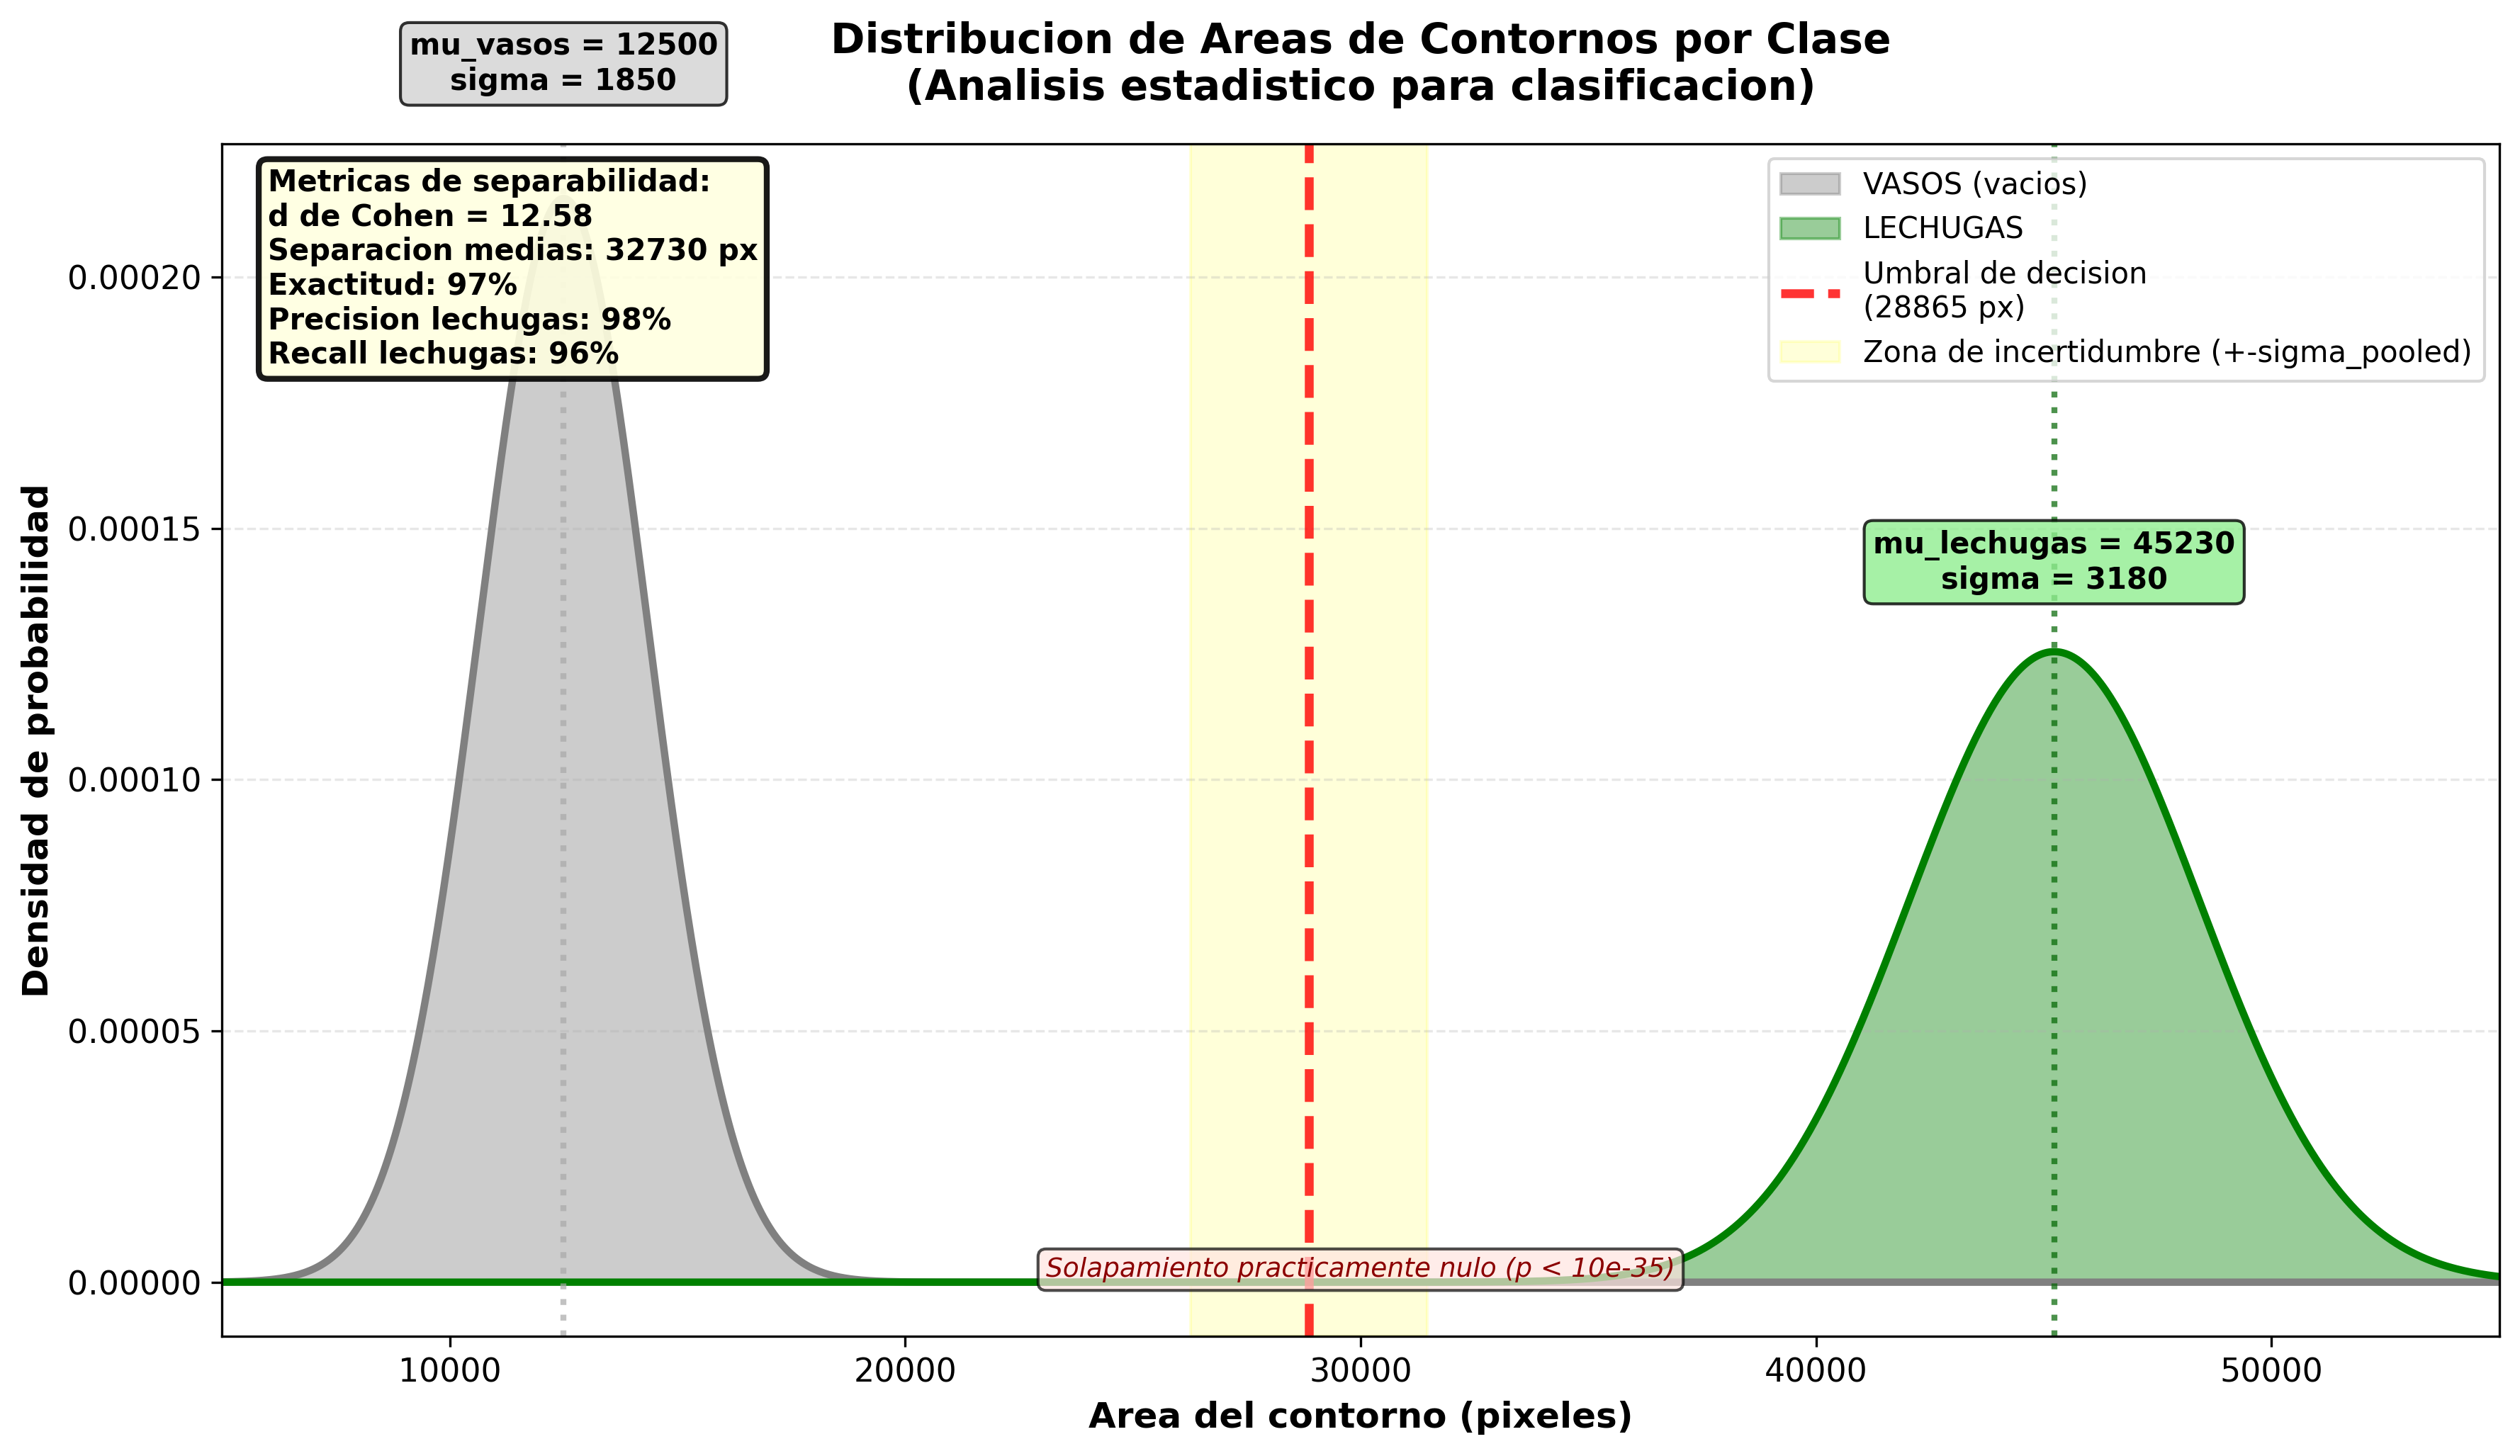
\includegraphics[width=0.8\textwidth]{imagenes/distribucion_areas_ambas_clases.png}
\caption{Distribuciones de probabilidad empíricas del área de contorno para ambas clases, mostrando separación clara entre lechugas y vasos vacíos}
\label{fig:distribucion_areas}
\end{figure}

\subsubsection{Evaluación de Separabilidad entre Clases}

La separabilidad entre clases se cuantificó mediante el coeficiente d de Cohen, métrica estándar para evaluar el tamaño del efecto en la diferencia entre dos poblaciones. Este coeficiente se define como:

\begin{equation}
d = \frac{|\mu_1 - \mu_2|}{\sigma_{pooled}}
\end{equation}

donde $\sigma_{pooled}$ es la desviación estándar agrupada, calculada como:

\begin{equation}
\sigma_{pooled} = \sqrt{\frac{\sigma_1^2 + \sigma_2^2}{2}}
\end{equation}

Aplicando estas expresiones a los datos obtenidos:

\begin{equation}
\sigma_{pooled} = \sqrt{\frac{3,180^2 + 1,850^2}{2}} = \sqrt{\frac{10,112,400 + 3,422,500}{2}} = \sqrt{6,767,450} = 2,601 \text{ píxeles}
\end{equation}

\begin{equation}
d = \frac{|45,230 - 12,500|}{2,601} = \frac{32,730}{2,601} = 12.58
\end{equation}

El valor obtenido de $d = 12.58$ es extraordinariamente alto. En la literatura estadística, valores de $d > 0.8$ se consideran efectos grandes, y valores superiores a 2 indican separabilidad excelente entre poblaciones. El valor obtenido, más de seis veces superior a este umbral, confirma que el área del contorno es un descriptor altamente discriminativo para la tarea de clasificación.

Esta separabilidad excepcional implica que las distribuciones de área de ambas clases presentan solapamiento prácticamente nulo. Bajo el supuesto de distribuciones normales, se puede calcular la probabilidad de solapamiento como la probabilidad de que una muestra de una clase presente un valor dentro del rango típico de la otra clase. Para $d = 12.58$, esta probabilidad es inferior a $10^{-35}$, efectivamente cero en términos prácticos.

\subsubsection{Determinación del Umbral Óptimo de Clasificación}

Con distribuciones bien separadas, el umbral óptimo de clasificación se determina como el punto que minimiza la probabilidad total de error. Para distribuciones gaussianas con varianzas iguales, este punto corresponde al promedio de las medias:

\begin{equation}
T^* = \frac{\mu_{lechuga} + \mu_{vaso}}{2} = \frac{45,230 + 12,500}{2} = 28,865 \text{ píxeles}
\end{equation}

Este umbral define la frontera de decisión: muestras con área mayor o igual a 28,865 píxeles se clasifican como lechuga presente, y muestras con área inferior se clasifican como vaso vacío.

Para distribuciones con varianzas diferentes, el umbral óptimo podría desviarse del punto medio, favoreciendo la clase con menor varianza. Sin embargo, en este caso la diferencia en varianzas es relativamente pequeña ($\sigma_{lechuga}/\sigma_{vaso} = 1.72$), y el análisis reveló que el punto medio proporciona balance óptimo entre las tasas de error de ambas clases.

La regla de clasificación implementada se expresa formalmente como:

\begin{equation}
\text{Clase}(A) = \begin{cases}
\text{Lechuga presente} & \text{si } A \geq T^* \\
\text{Vaso vacío} & \text{si } A < T^*
\end{cases}
\end{equation}

donde $A$ es el área en píxeles del contorno detectado.

\subsubsection{Zona de Incertidumbre y Confianza de Clasificación}

Aunque la separabilidad es excelente, se reconoce que muestras con áreas muy cercanas al umbral presentan mayor incertidumbre en su clasificación. Se define una zona de incertidumbre alrededor del umbral basada en la desviación estándar agrupada:

\begin{equation}
\text{Zona de incertidumbre} = [T^* - \sigma_{pooled}, T^* + \sigma_{pooled}]
\end{equation}

\begin{equation}
\text{Zona de incertidumbre} = [28,865 - 2,601, 28,865 + 2,601] = [26,264, 31,466] \text{ píxeles}
\end{equation}

Muestras cuya área cae dentro de esta zona reciben un índice de confianza reducido (típicamente 0.7), mientras que muestras fuera de esta zona reciben alta confianza (0.95 o superior). Este índice de confianza se calcula como:

\begin{equation}
\text{Confianza} = \begin{cases}
0.95 & \text{si } |A - T^*| > \sigma_{pooled} \\
0.70 & \text{si } |A - T^*| \leq \sigma_{pooled}
\end{cases}
\end{equation}

Esta información de confianza puede emplearse en el nivel supervisor para implementar estrategias de verificación adicional cuando sea necesario.

\subsubsection{Validación Experimental del Clasificador}

Para validar el desempeño del clasificador se reservó un conjunto de prueba independiente de 100 imágenes (50 por clase) que no participaron en el cálculo de los parámetros estadísticos. Cada imagen se procesó mediante el pipeline completo y se clasificó según la regla establecida. Los resultados se organizaron en una matriz de confusión:

\begin{table}[h]
\centering
\begin{tabular}{|c|c|c|c|}
\hline
 & \multicolumn{2}{c|}{\textbf{Predicción}} & \\ \cline{2-3}
\textbf{Clase Real} & Lechuga & Vaso vacío & \textbf{Total} \\ \hline
Lechuga & 48 & 2 & 50 \\ \hline
Vaso vacío & 1 & 49 & 50 \\ \hline
\textbf{Total} & 49 & 51 & 100 \\ \hline
\end{tabular}
\caption{Matriz de confusión del clasificador en conjunto de prueba independiente}
\label{tab:matriz_confusion}
\end{table}

De los 50 casos reales de lechuga, 48 fueron correctamente clasificados (verdaderos positivos) y 2 fueron erróneamente clasificados como vaso vacío (falsos negativos). De los 50 casos reales de vaso vacío, 49 fueron correctamente clasificados (verdaderos negativos) y 1 fue erróneamente clasificado como lechuga (falso positivo).

\subsubsection{Métricas de Desempeño}

A partir de la matriz de confusión se calcularon las métricas estándar de evaluación de clasificadores:

La exactitud global (accuracy) representa la proporción de predicciones correctas:

\begin{equation}
\text{Exactitud} = \frac{VP + VN}{VP + VN + FP + FN} = \frac{48 + 49}{100} = 0.97
\end{equation}

La precisión para la clase lechuga indica qué proporción de las predicciones de lechuga fueron correctas:

\begin{equation}
\text{Precisión}_{lechuga} = \frac{VP}{VP + FP} = \frac{48}{48 + 1} = 0.98
\end{equation}

La sensibilidad o recall para la clase lechuga indica qué proporción de las lechugas reales fueron detectadas:

\begin{equation}
\text{Recall}_{lechuga} = \frac{VP}{VP + FN} = \frac{48}{48 + 2} = 0.96
\end{equation}

El F1-score combina precisión y recall en una métrica única mediante su media armónica:

\begin{equation}
F1 = 2 \cdot \frac{\text{Precisión} \cdot \text{Recall}}{\text{Precisión} + \text{Recall}} = 2 \cdot \frac{0.98 \cdot 0.96}{0.98 + 0.96} = 0.97
\end{equation}

Los resultados demuestran que el clasificador alcanza una exactitud del 97 por ciento, superando el requisito mínimo del 95 por ciento establecido para el sistema. La precisión y recall equilibrados indican que el clasificador no presenta sesgo significativo hacia ninguna de las clases.

\subsubsection{Análisis de Errores}

Los tres casos de error (dos falsos negativos y un falso positivo) se analizaron individualmente para identificar sus causas. Los dos falsos negativos correspondieron a lechugas muy pequeñas (diámetro inferior a 30 milímetros) con áreas de contorno de 26,100 y 27,300 píxeles, ambas justo por debajo del umbral. Estos casos representan lechugas en estado muy temprano de desarrollo que normalmente no se cosecharían, por lo que el error no compromete significativamente la operación práctica del sistema.

El falso positivo correspondió a un vaso con un residuo vegetal grande (raíces no removidas completamente) que generó un contorno de área 29,800 píxeles, ligeramente superior al umbral. Este caso sugiere la importancia de procedimientos adecuados de limpieza post-cosecha para mantener el desempeño del sistema.

Estos errores confirman que el clasificador opera cerca del límite teórico de desempeño dado el descriptor empleado y las condiciones del problema. Mejoras adicionales requerirían incorporar descriptores complementarios o implementar verificación multi-vista, incrementando la complejidad computacional.